\documentclass[10pt,dvipdfm]{beamer}

\usepackage{hcystyle}

%%%%%%%文档正文
\begin{document}

%标题作者等信息。
%这些信息将自动生成ppt的第一页
\title[毕业设计答辩]{\LARGE{毕业设计答辩\\}}
%\subtitle{基于动态链接技术的{\cp web}服务器动态扩展功能\\接口的设计与实现}
\author[黄丛宇]{黄丛宇\\06161032\\指导老师:马瑞芳}
\institute[西安交通大学 软件学院]{西安交通大学 软件学院 软件62班}
\date{\today}

\begin{frame}	
	\titlepage
\end{frame}

\begin{frame}
	\frametitle{目录}
	\tableofcontents
\end{frame}

\section{课题名称}
%第二页
\begin{frame}
	\frametitle{课题名称}
	
	\begin{block}{}
	\begin{center}
	{\Large
			基于动态链接技术的web服务器动态扩展功能\\
				接口的设计与实现
	}
	\end{center}
	\end{block}
	
\end{frame}

\section{背景和意义}

\begin{frame}
	\frametitle{背景和意义}
	\begin{center}
	{\Large
		一、背景和意义
	}
	\end{center}
\end{frame}

\begin{frame}
	\frametitle{背景和意义}
	\begin{block}{Web服务器:}
		\begin{itemize}
			\item[-] 互联网的核心组成部分,支撑整个互联网应用服务。
			\item[-] 适应互联网应用的不断更新变化。
			\item[-] 必须保证7*24小时的运行。
		\end{itemize}
	\end{block}
	
	\pause
	
	\begin{block}{Web服务器现状:}
		\begin{itemize}
			\item[*] 大部分都不支持功能的动态增加。
			\item[*] 必须重启或重新编译。
		\end{itemize}
	\end{block}
	
\end{frame}

\begin{frame}
	\frametitle{背景和意义}
	\begin{block}{}
	\begin{itemize}
		\item 针对以上问题,本课题将基于动态链接库技术,使服务器在运行期间,可以动态的获知模块的增加并加载模块。
		\item 本系统实现了服务器的基本功能,重点实现模块动态加载特性。
	\end{itemize}
	\end{block}
\end{frame}

\section{HTTP协议分析}

\begin{frame}
	\frametitle{HTTP协议分析}
	\begin{center}
	{\Large
		二、HTTP协议分析
	}
	\end{center}
\end{frame}

\begin{frame}
	\frametitle{HTTP协议简介}
	
HTTP协议(Hypertext Transfer Protocol,超文本传输协议)是一个属于应用层的面向对象的协议。它于1990年提出。主要用于从WWW服务器传输超文本到本地浏览器的传送协议。

 	\pause

\begin{block}{HTTP协议具有如下特点:}
\five{
	\begin{enumerate}
		\item 支持客户/服务器模式。
		\item 简单快速:客户向服务器请求服务时,只需传送请求方法和路径。
		\item 灵活:HTTP允许传输任意类型的数据对象。
		\item 无连接:无连接的含义是限制每次连接只处理一个请求。
		\item 无状态:协议对于事务处理没有记忆能力。
	\end{enumerate}
}
\end{block}
\end{frame}

\begin{frame}
	\frametitle{HTTP协议处理过程}
	\begin{figure}[htbp]
	\centering
	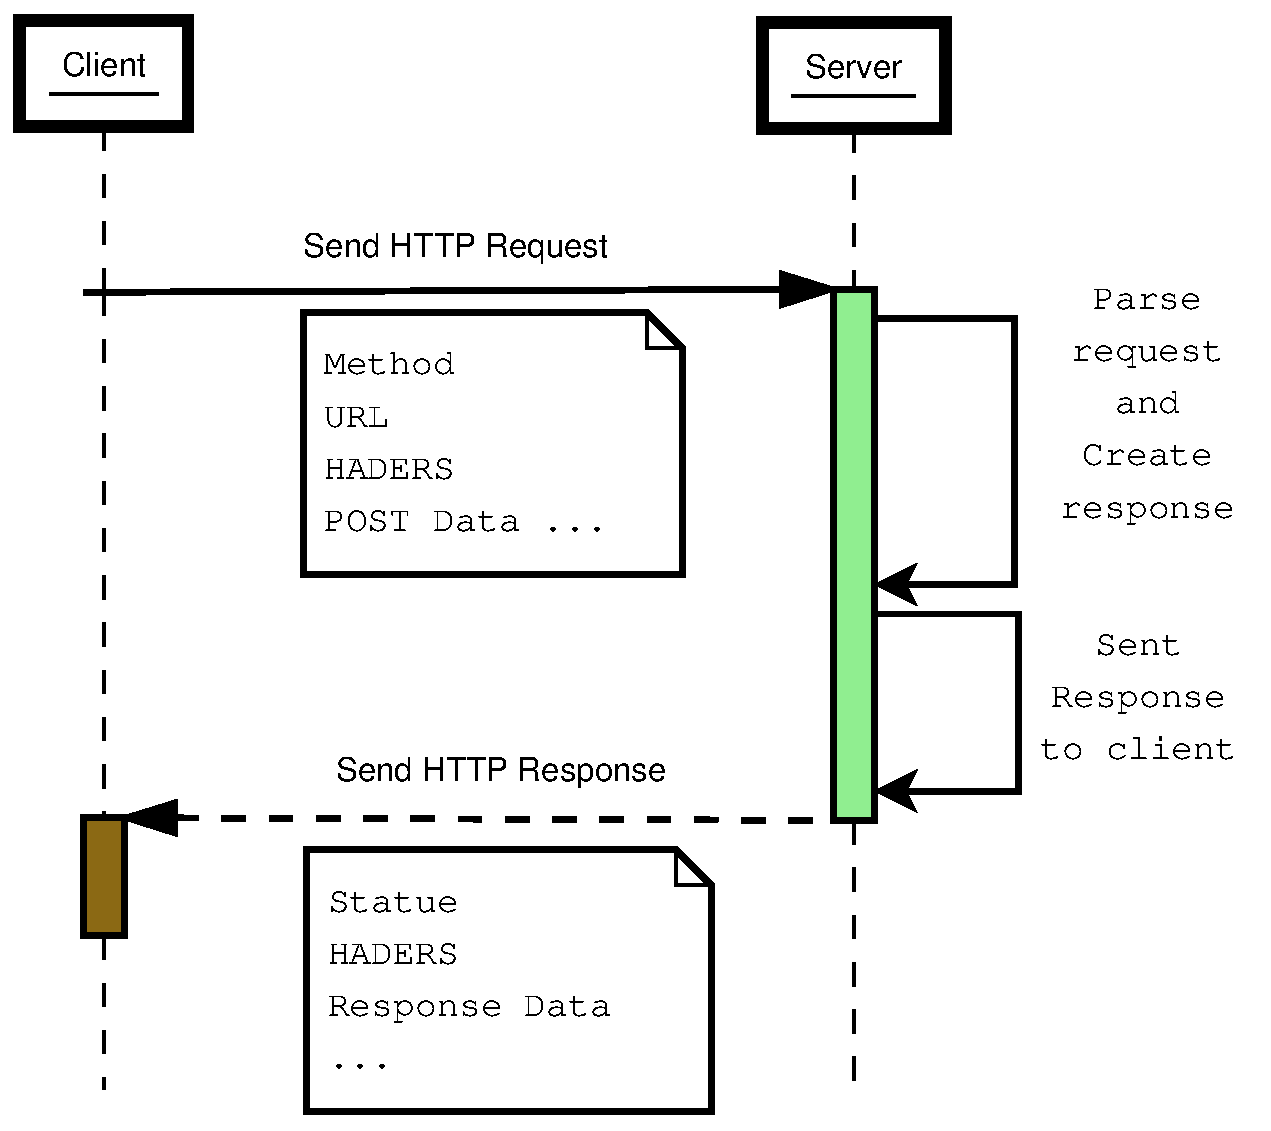
\includegraphics[height=6cm, width=7cm]{http.eps}
	\end{figure}
\end{frame}

%要使用verbatim环境,必须是这个格式。begin{frame}不可以。
\frame[containsverbatim]{
	\frametitle{Request格式}
	
	{\scriptsize
	\begin{verbatim}
        ---------------------------------------
        | Methods |sp| URL |sp| Version |cr|lf|  -----> Request line
        ---------------------------------------
        | Header Field Name: |sp| Value |cr|lf|  -]
        ---------------------------------------   |
        |   ... (more headers)                |   |---> Header lines
        ---------------------------------------   |
        | Header Field Name: |sp| Value |cr|lf|  -]
        ---------------------------------------
        |cr|lf|                                  -----> a blank line
        ---------------------------------------
        |                                     |
        | Data...                             |  -----> Entity body
        |                                     |
        ---------------------------------------
        cr = \r ; lf = \n ; sp = blankspace
 	\end{verbatim}
 	}%\scriptsize
 	
 	\begin{block}{}
 	此格式规定了HTTP协议中每一个Request中数据的意义。服务器根据此格式理解请求的内容。
 	\end{block}
}

\begin{frame}
	\frametitle{需要处理的HEADERS}
	\begin{block}{HEADERS:}
	\begin{enumerate}[(a)]
		\item Connection: 标记是否保持连接。
		\item Content-Length: POST数据的长度。
		\item Content-Type: POST数据的格式。
		\item Host: 主机名。HTTP/1.1要求必须有主机名。
		\item If-Modifice-Since: 用于缓存。
		\item If-None-Match: 用于缓存。
	\end{enumerate}
	\end{block}
\end{frame}

\section{插件接口设计}

\begin{frame}
	\frametitle{插件接口设计}
	\begin{center}
	{\Large
		三、插件接口设计
	}
	\end{center}
\end{frame}

\begin{frame}
	\frametitle{插件动态加载过程}
	
	服务器通过实时监测插件配置文件是否修改。一旦监测到修改,立即加载(卸载)插件。
	
	\pause
	
	\begin{block}{处理过程如下:}
	\begin{figure}[htbp]
	\centering
	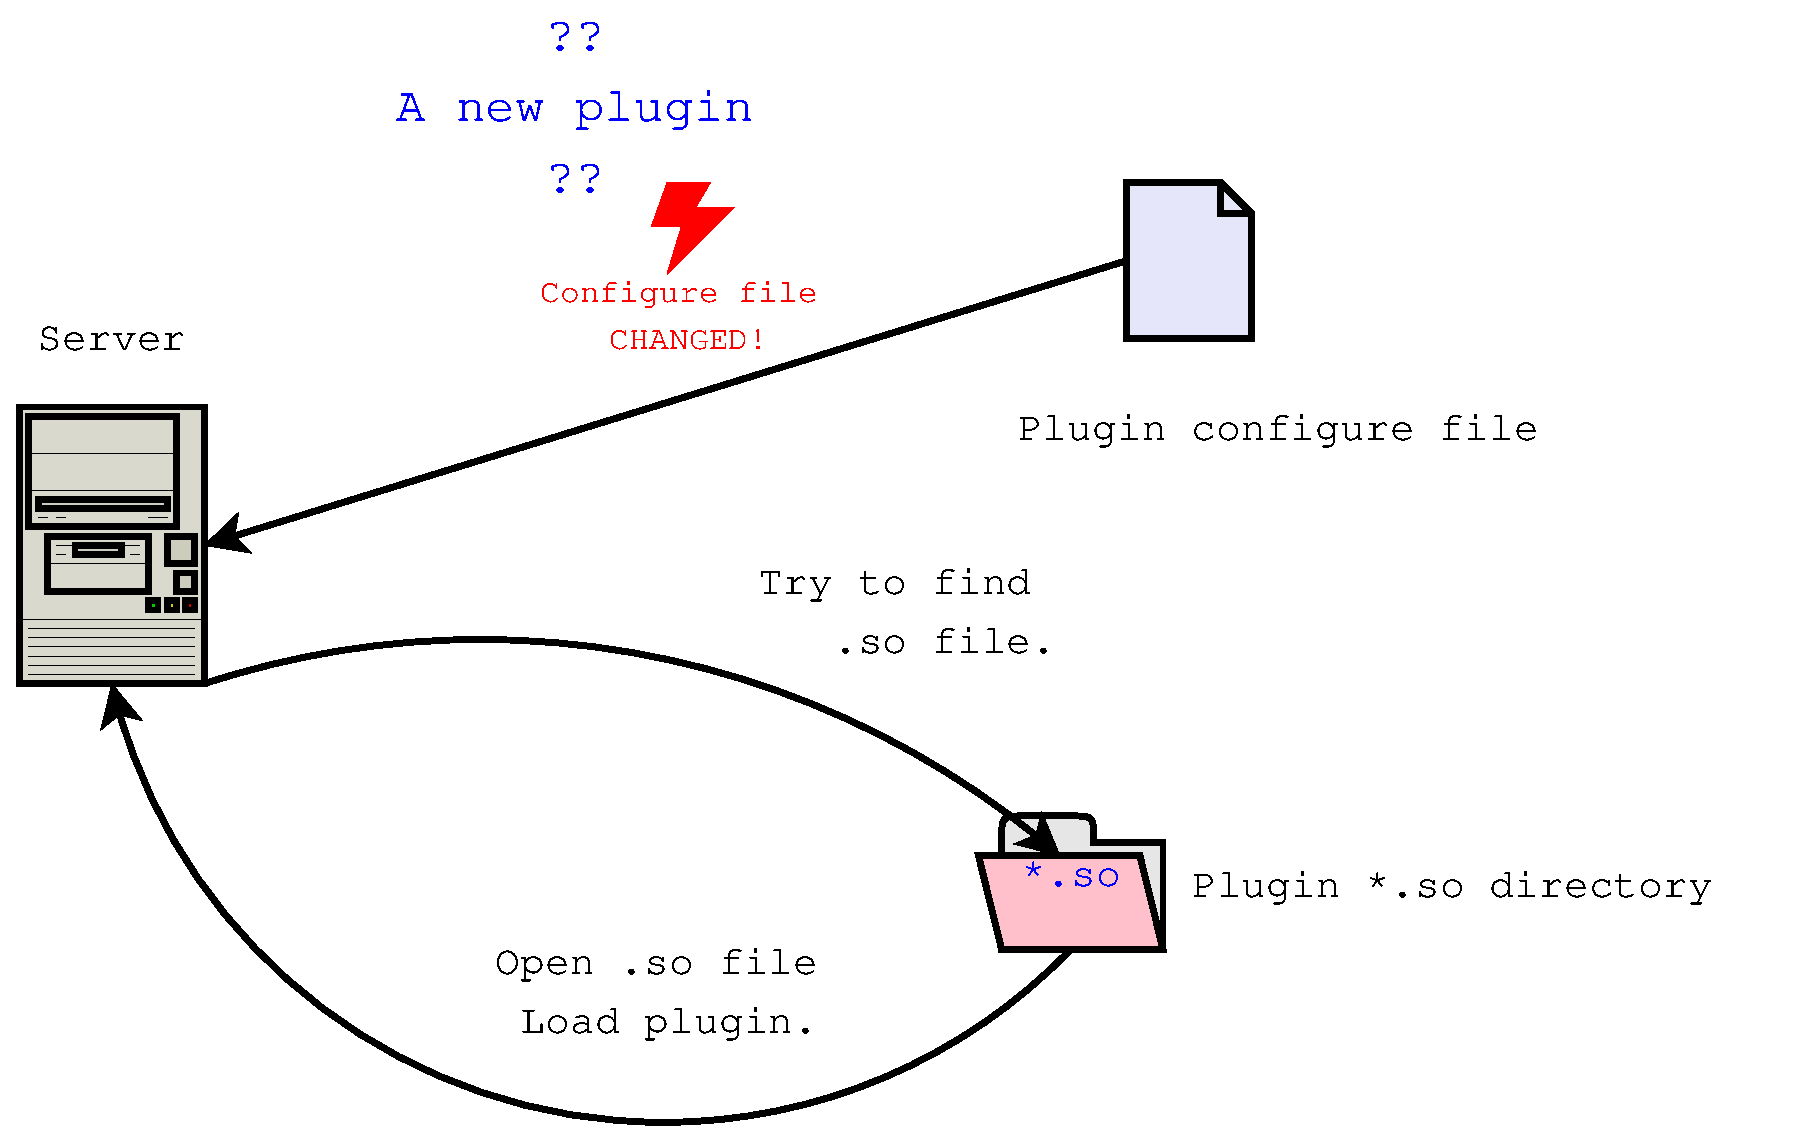
\includegraphics[height=5cm, width=9cm]{loadplugin.eps}
	\end{figure}
	\end{block}
\end{frame}

\begin{frame}
	\frametitle{插件调用过程}
	服务器对HTTP协议Request数据进行解析。	在解析的过程中调用插件对Request进行处理。
	
	\pause
	
	\begin{block}{处理过程如下:}
	\begin{figure}[htbp]
	\centering
	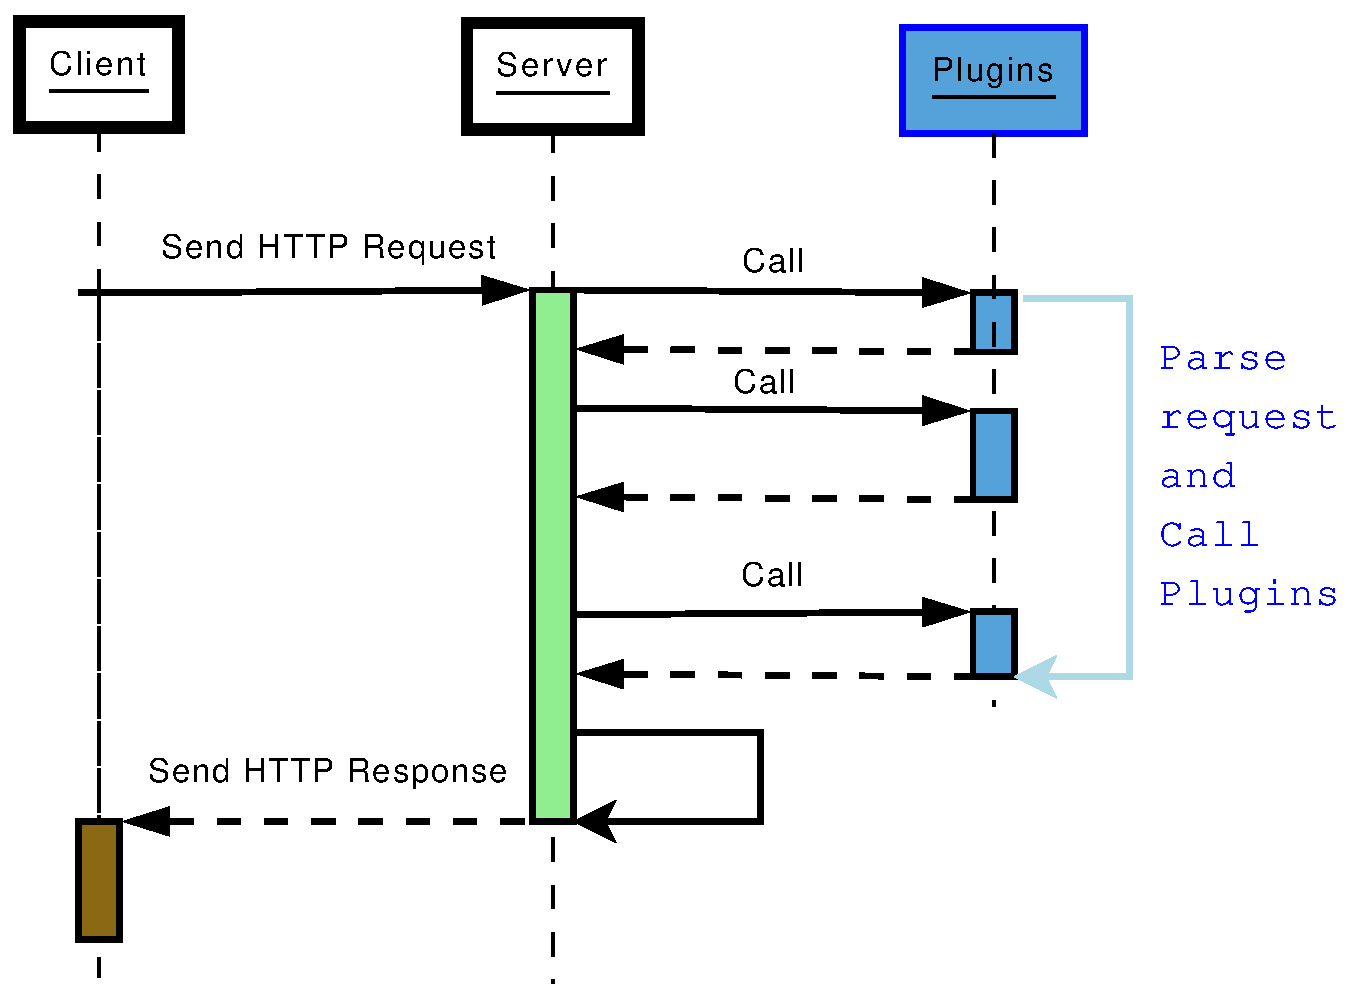
\includegraphics[height=5cm, width=8cm]{httpplugin.eps}
	\end{figure}
	\end{block}
\end{frame}


\begin{frame}
	\frametitle{插件接口定义:}
	接口定义一些列函数原型。所有函数都有明确的定义和调用时机。
	
	插件选择性的实现这些函数。服务器在确定的时机调用所有插件的对应函数。
	
	\pause
	
	\begin{block}{接口定义:}
	\begin{itemize}
		\item[-] init: 初始化插件。
		\item[-] set\_default: 设置插件的配置为默认值。
		\item[-] cleanup: 清理插件。
		\item[-] trigger: 每秒钟调用一次。相当于计时器。
		\item[-] sighup: 处理挂断信号。
	\end{itemize}
	\end{block}
\end{frame}

\begin{frame}
	\frametitle{插件接口定义:}
	\begin{block}{接口定义(续):}
	\begin{itemize}
		\item[-] url\_raw: 获得未解码的URL地址后调用。
		\item[-] url\_clean: 获得已解码的URL地址后调用。
		\item[-] docroot: 设置插件工作的根目录 。
		\item[-] physical: 获得请求资源对应的物理地址后调用。
		\item[-] connection\_close: 连接关闭时调用。
		\item[-] connection\_reset: 连接重置时调用。
		\item[-] joblist: 连接被加入joblist时调用嗯。
		\item[-] subrequest\_start: 子请求开始。
		\item[-] handle\_subrequest: 处理子请求。
		\item[-] subrequest\_end: 子请求结束。
	\end{itemize}
	\end{block}
\end{frame}

\section{服务器设计}

\begin{frame}
	\frametitle{服务器设计}
	\begin{center}
	{\Large
		四、服务器设计
	}
	\end{center}
\end{frame}

\begin{frame}
	\frametitle{IO设计}
	\begin{columns}
		\begin{column}{0.25\textwidth}
			\begin{alertblock}{}
				Nonblocking IO
			\end{alertblock}
			
		\end{column}
		
		\begin{column}{0.02\textwidth}
			\begin{alertblock}{}
				+
			\end{alertblock}
		\end{column}
		
		\begin{column}{0.28\textwidth}
			\begin{alertblock}{}
				IO multiplexing
			\end{alertblock}
			
		\end{column}
		
		\begin{column}{0.02\textwidth}
			\begin{alertblock}{}
				+
			\end{alertblock}
		\end{column}
		
		\begin{column}{0.22\textwidth}
			\begin{alertblock}{}
				Thread pool
			\end{alertblock}
		\end{column}
	\end{columns}
	\pause
	\begin{block}{IO结构图:}
	\begin{figure}[htbp]
	\centering
	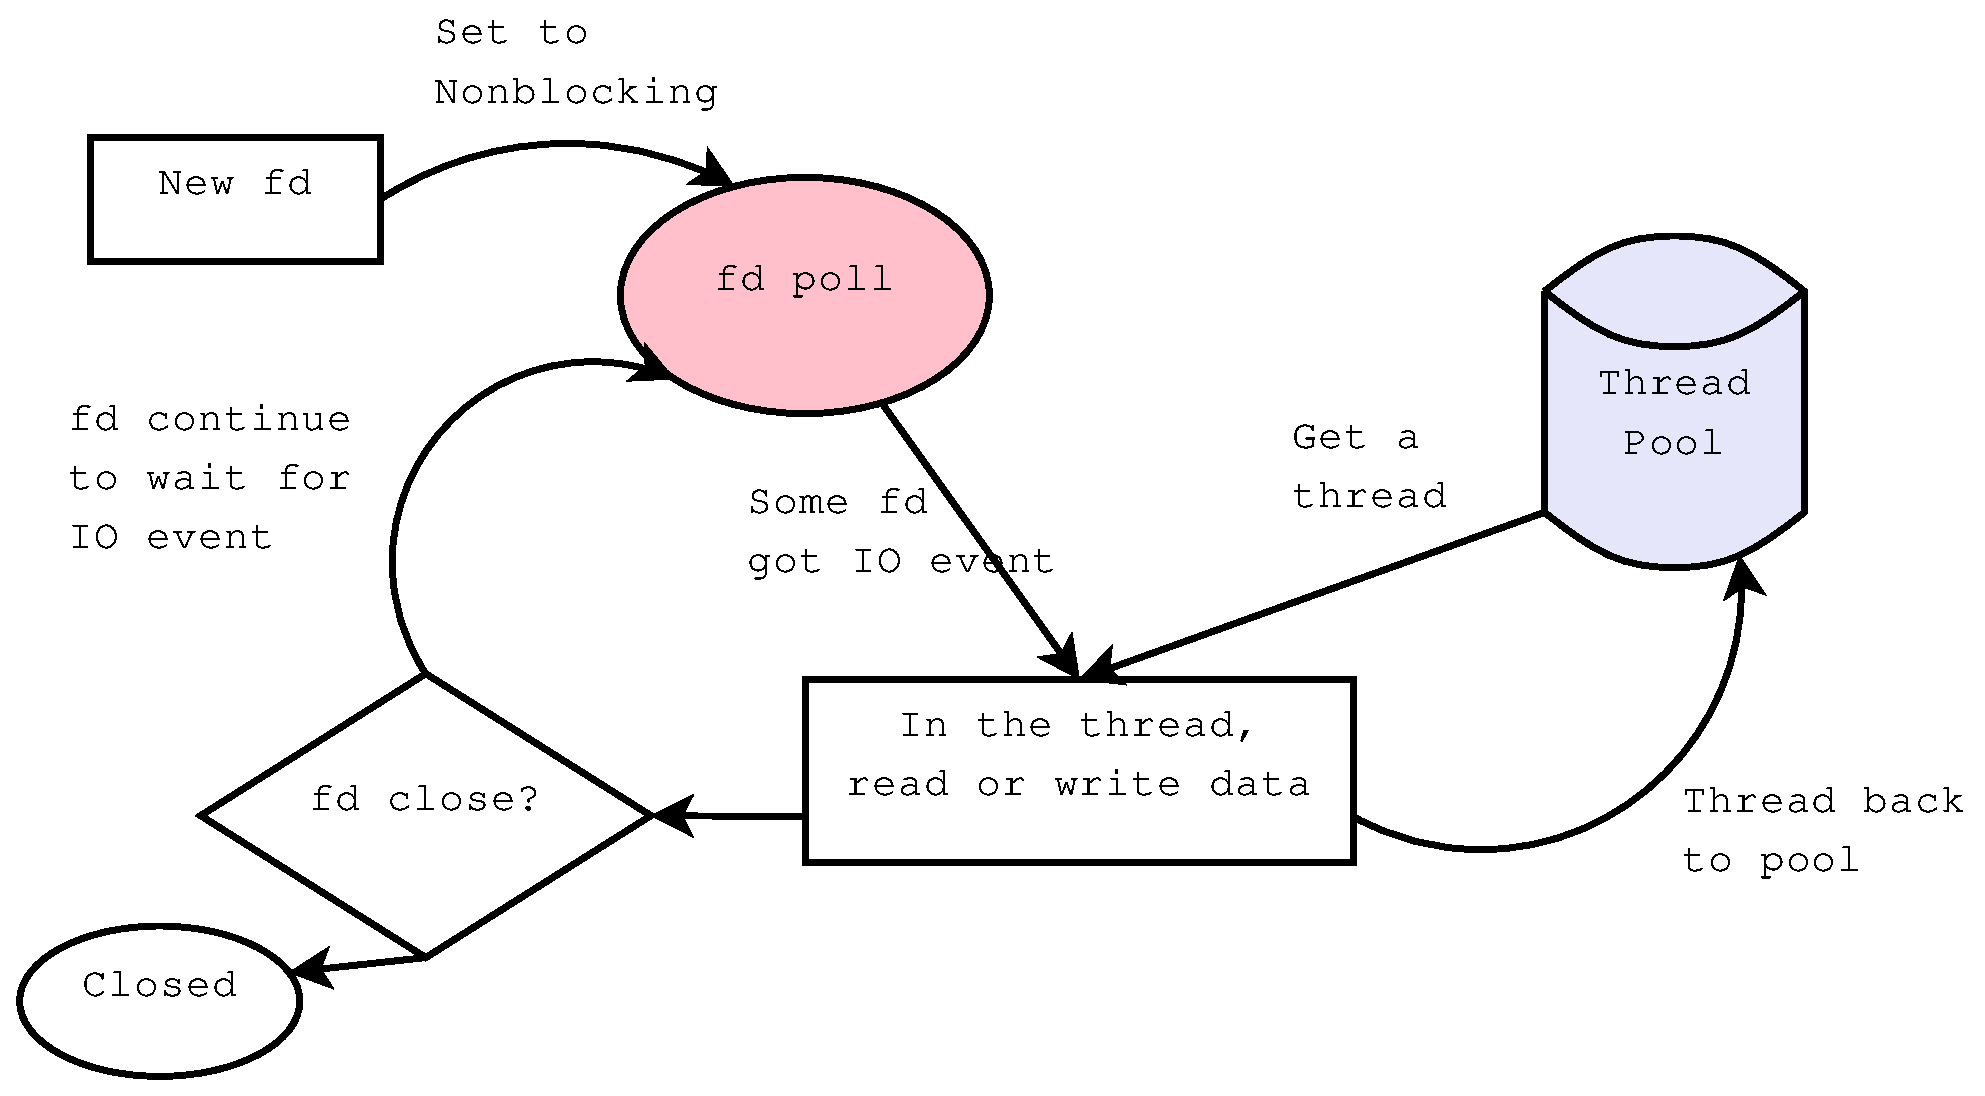
\includegraphics[height=5cm, width=10cm]{IO.eps}
	\end{figure}
	\end{block}
	
\end{frame}


\begin{frame}
	\frametitle{连接处理:状态机}
	使用状态机对连接进行处理。
	
	对连接定义一系列状态。在整个生命周期中,连接处于某一个状态。根据连接的当前状态和所发生的事件,使连接进入下一状态。
	
	\pause
	
	\begin{example}{例如:}
	\begin{figure}[htbp]
	\centering
	\includegraphics[height=3cm, width=4cm]{statemachine.eps}
	\end{figure}
	\end{example}
\end{frame}

\section{插件接口实现}

\begin{frame}
	\frametitle{插件接口实现}
	\begin{center}
	{\Large
		五、插件接口实现
	}
	\end{center}
\end{frame}

\frame[containsverbatim]{
	\frametitle{接口实现}
	\begin{block}{主要的数据结构:}
		\begin{enumerate}
			\item plugin\_slot\_t枚举类型
			\item plugin结构体
			\item plugin\_slot结构体。
		\end{enumerate}
	\end{block}
	plugin\_slot\_t枚举类型用于定义接口函数的类型。与接口函数一一对应。
	\begin{example}
	\begin{verbatim}
	PLUGIN_SLOT_SET_DEFAULT
	PLUGIN_SLOT_CLEANUP
	PLUGIN_SLOT_TRIGGER
	PLUGIN_SLOT_URL_RAW
	PLUGIN_SLOT_URL_CLEAN
	...
	\end{verbatim}
	\end{example}
}

\begin{frame}
	\frametitle{接口实现}
	plugin结构体包含一个插件的所有信息。包括版本,名称以及一系列接口函数的地址。plugin结构体类似于一个类。服务器通过调用其成员方法(函数指针)来执行插件的功能。
	
	定义如下:
	\begin{figure}[htbp]
	\centering
	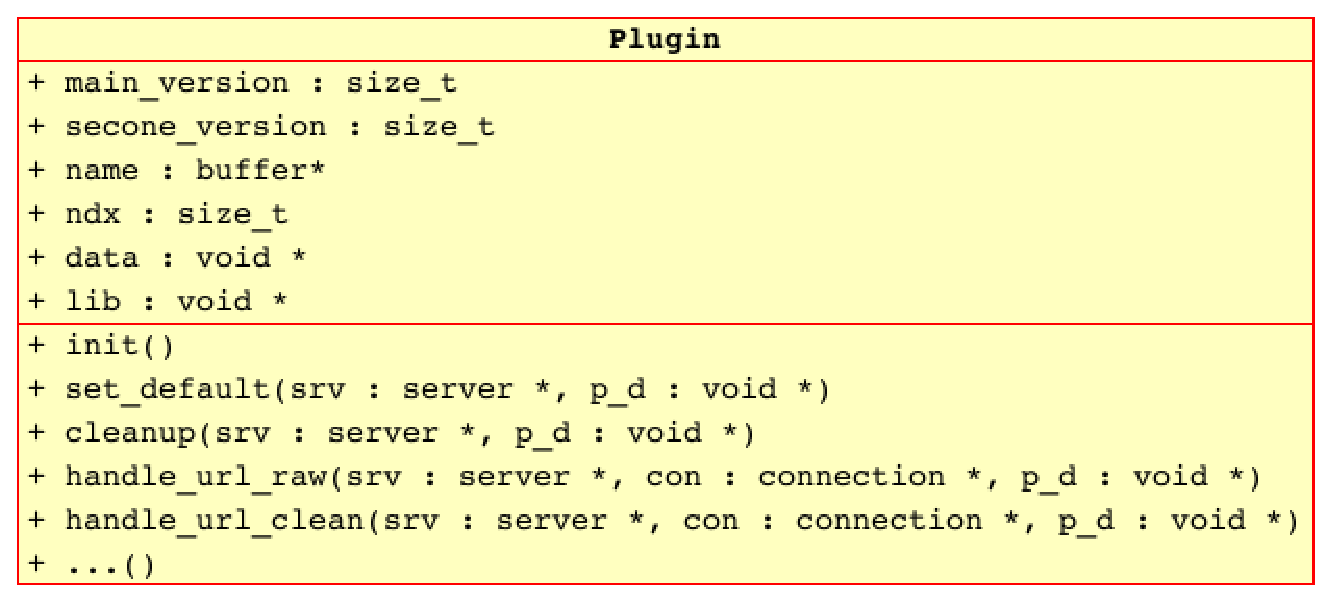
\includegraphics[height=4cm, width=8cm]{plugin_s.eps}
	\end{figure}
\end{frame}

\begin{frame}
	\frametitle{接口实现}
	plugin\_slot是一个二维数组。相当于plugin的登记表。服务器通过这个表中的信息对插件进行调用。
	表的形式如下:
	\begin{table}[htbp]
	\caption{plugin\_slot示例:}
	\centering
	\begin{tabular}{cccc} %最后一列是空的。这样可以是倒数第二列居中,否则会报错或不居中。
	\toprule
	\centering 名称 & 插件1 & 插件2 &插件3\\
	\midrule
	\centering PLUGIN\_SLOT\_URL\_RAW & p1 &  p2 & p3\\
	\centering PLUGIN\_SLOT\_URL\_CLEAN &  p1 &  NULL & p3\\
	\centering PLUGIN\_SLOT\_DOCROOT & p1 & NULL & NULL\\
	\bottomrule
	\end{tabular}
	\end{table}
	\begin{block}{}
		表中存放的是plugin结构体指针。NULL表示此插件没有实现这个函数。
	\end{block}
\end{frame}

\begin{frame}
	\frametitle{接口实现}
	服务器中包含一个定义插件的配置文件: swiftd-plugin.conf。
	
	\begin{block}{配置文件的形式如下:}	
		\#swiftd-plugin.conf
		\#配置文件的形式为  -- 插件名称:插件动态库文件所在目录\$\\
		\#每个插件一行,每个插件配置信息必须以"\$"结尾。\\
		dir\_index:/home/hcy/plugins/\$\\
		...
	\end{block}
	
	\pause
	
	\begin{block}{}
	动态库文件的名称为: \textcolor{read}{插件名称 + .so}。\\
	服务器通过监测这个配置文件,确定是否有插件需要加载或删除。
	\end{block}
\end{frame}

\begin{frame}
	\frametitle{接口实现}
	服务器使用inotify监测插件配置文件。inotify产生一个文件描述符,通过监测这个文件描述符是否有数据可读即可监测到文件的改变。
	\begin{block}{监测的过程如下:}
	\begin{figure}[htbp]
	\centering
	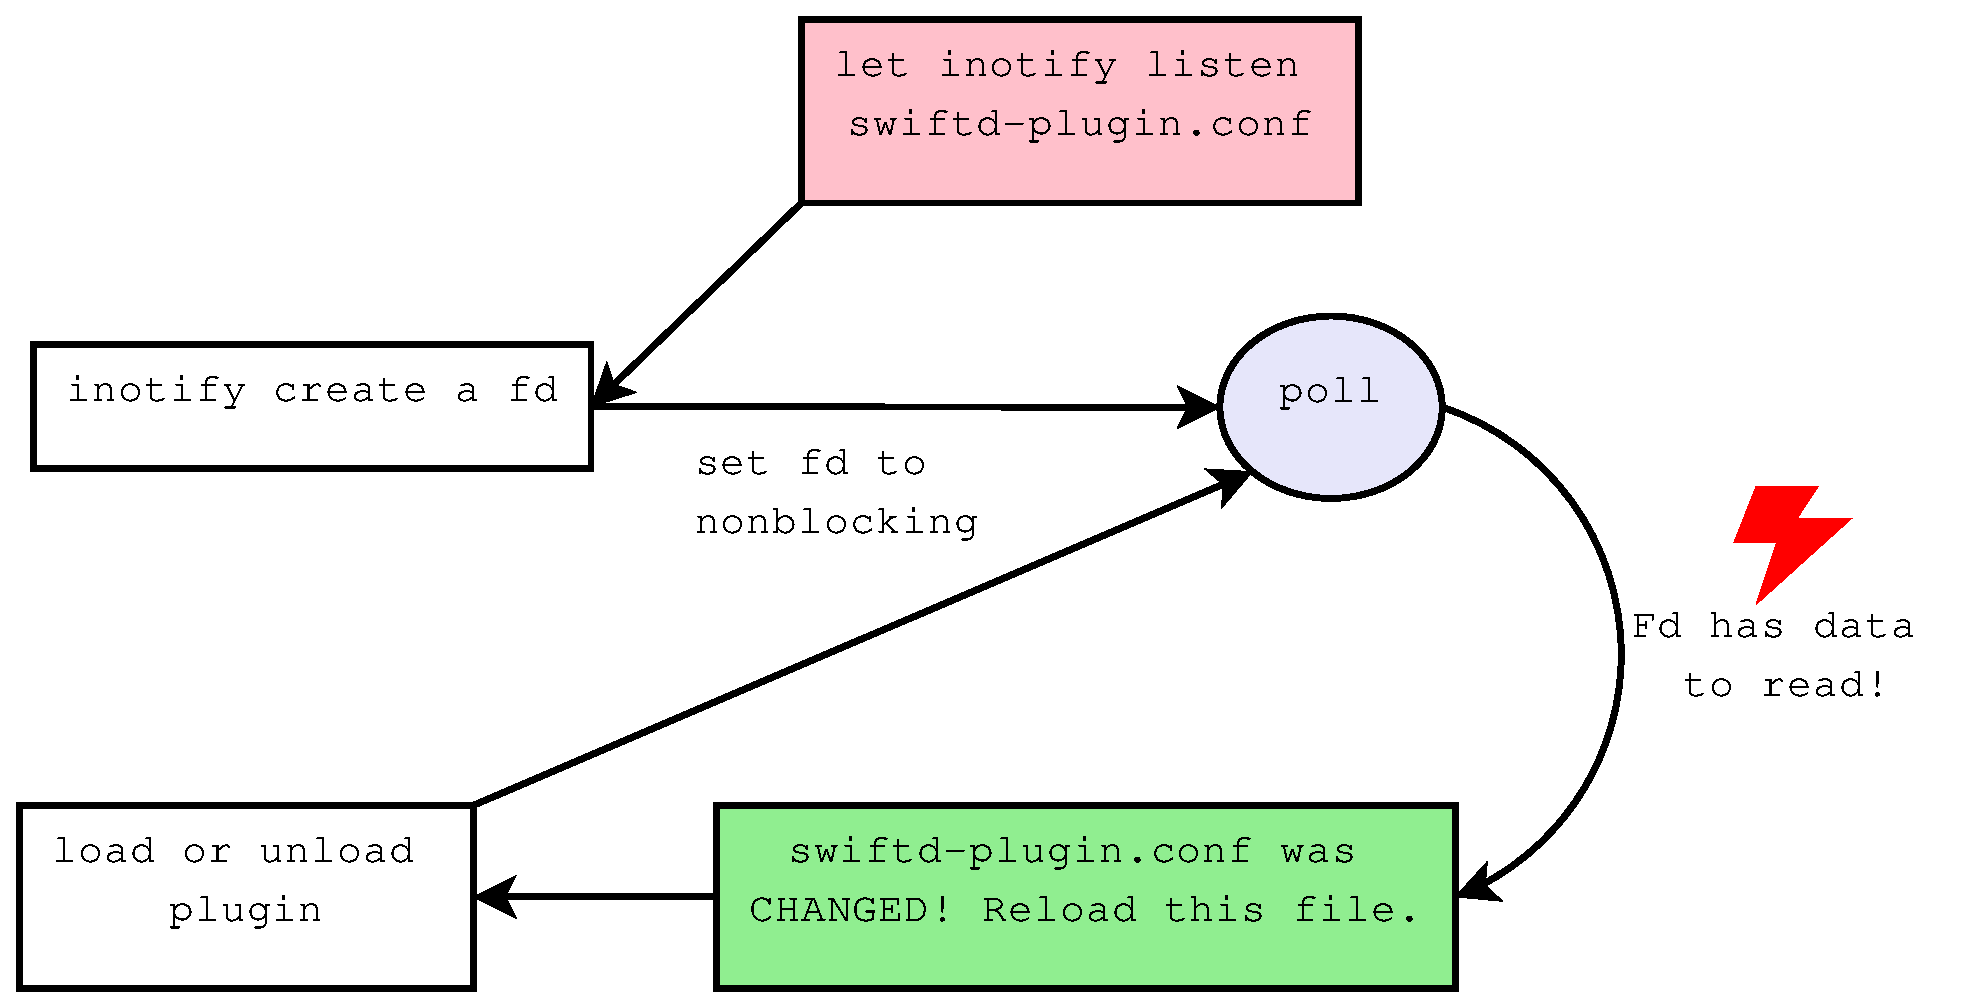
\includegraphics[height=5cm, width=9cm]{inotify.eps}
	\end{figure}
	\end{block}
\end{frame}

\section{服务器实现}

\begin{frame}
	\frametitle{服务器实现}
	\begin{center}
	{\Large
		六、服务器实现
	}
	\end{center}
\end{frame}

\begin{frame}
	\frametitle{IO实现}
	使用epoll对文件描述符的IO事件进行监测。
	
	
	每个文件描述符都有一个对应的IO事件处理函数。一旦有IO事件发生,申请一个线程,在线程中调用这个函数处理IO事件。
	\pause
	\begin{block}{IO事件处理过程:}
	\begin{figure}[htbp]
	\centering
	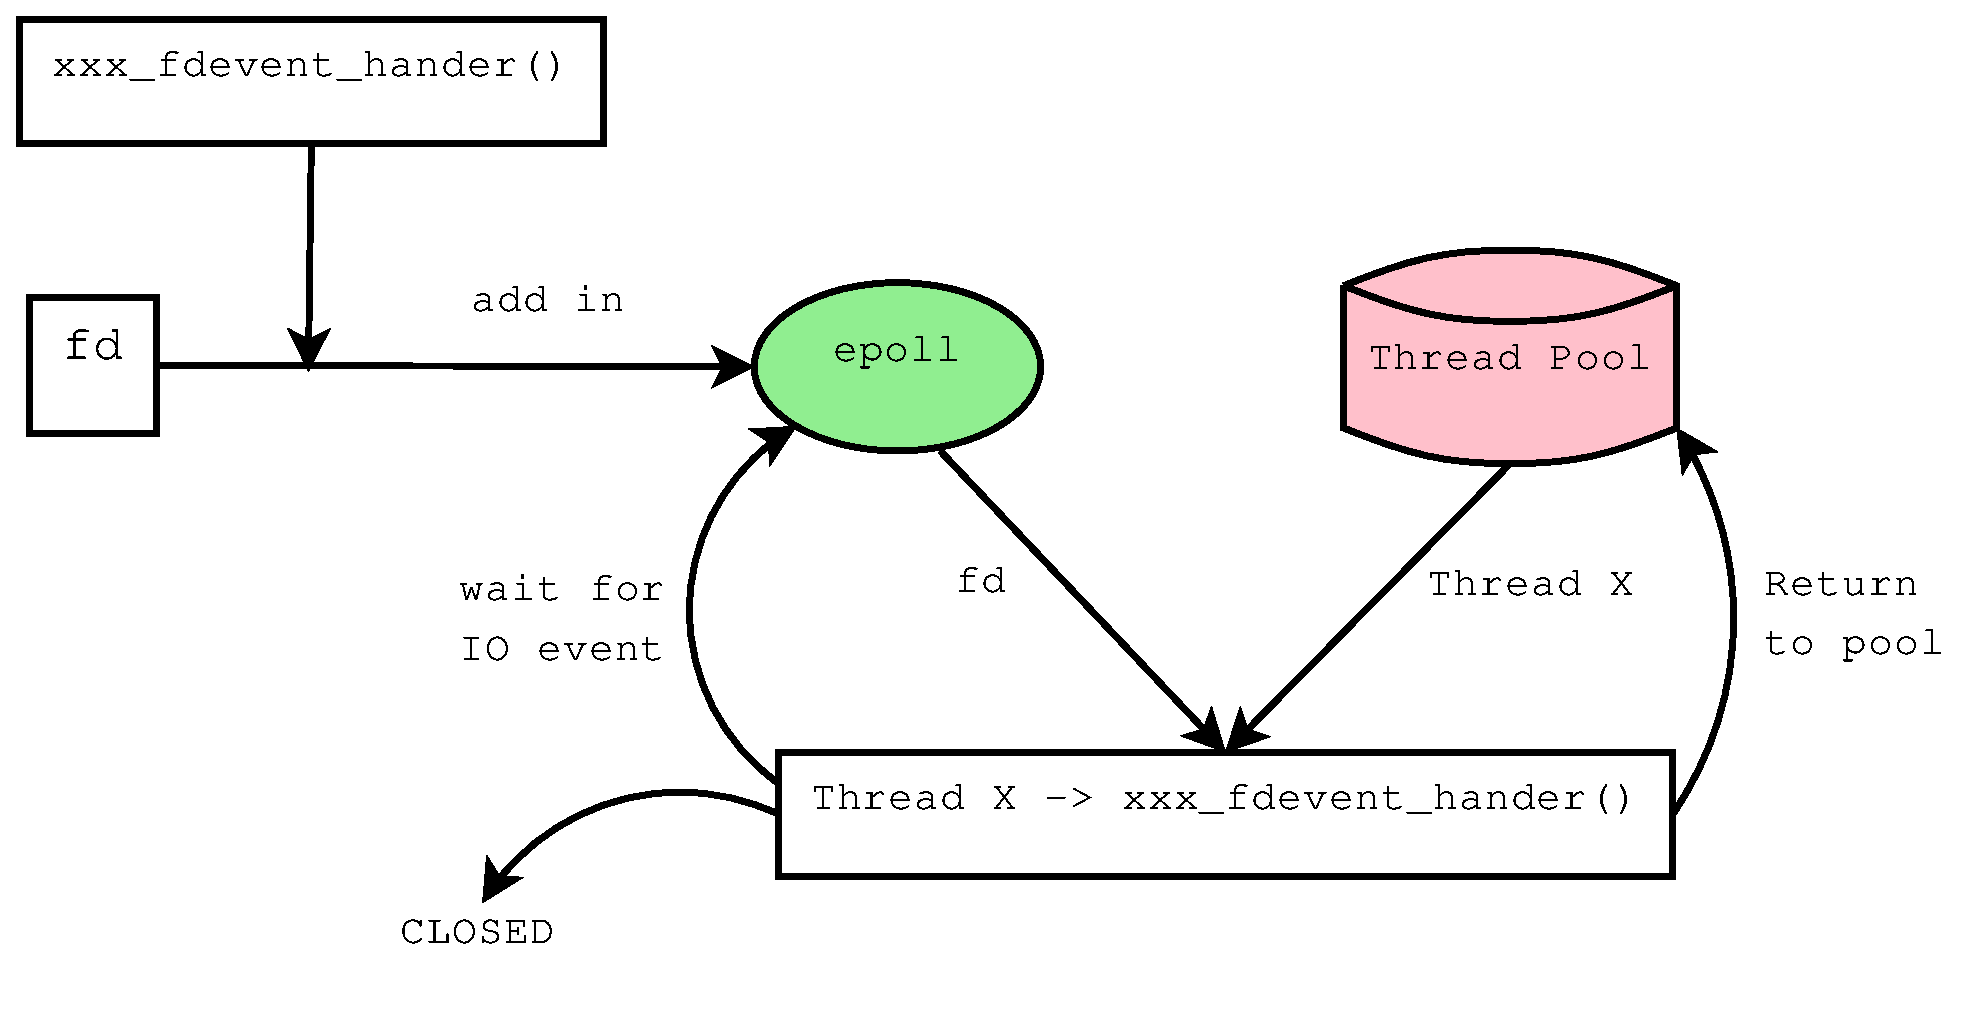
\includegraphics[height=5cm, width=9cm]{epoll.eps}
	\end{figure}
	\end{block}
	
\end{frame}

\begin{frame}
	\frametitle{IO实现}
	\begin{block}{Queue}
		每个连接对应三个队列。用来存储数据:
		\begin{enumerate}
			\item read\_queue : 读取的数据,要加锁。
			\item write\_queue : 发送的数据
			\item requet\_content\_queue : POST数据
		\end{enumerate}
	\end{block}
	\pause
	\begin{block}{线程池}
		每个线程的主循环中,调用传递进来的函数。(包括参数)\\
		使用pthread的条件变量对线程进行唤醒和睡眠操作。\\
		预先创建线程。提高效率。
	\end{block}
\end{frame}

\begin{frame}
	\frametitle{连接处理的状态机}
	对于每个连接,在其生存周期中,共定义了11个状态。
	
	
	\begin{block}{连接状态:}
		\begin{itemize}
			\item connect: 标记connection结构体可用。
			\item requeststart: 请求开始。
			\item read: 读取Request数据。
			\item handlerequest: 解析Request数据。
			\item requestend: 解析结束。
		\end{itemize}
	\end{block}
\end{frame}

\begin{frame}
	\frametitle{连接处理的状态机}
	\begin{block}{连接状态(续):}
		\begin{itemize}
			\item readpost: 读取POST数据。
			\item responsestart: 处理请求。在这个状态中调用插件。
			\item write: 发送数据回client。
			\item responseend: 处理结束。
			\item error: 出错。
			\item close: 连接关闭。
		\end{itemize}
	\end{block}
\end{frame}

\begin{frame}
	\begin{columns}
	
	\begin{column}{0.6\textwidth}
		\frametitle{连接处理的状态机}
		\begin{figure}[htbp]
		\centering
		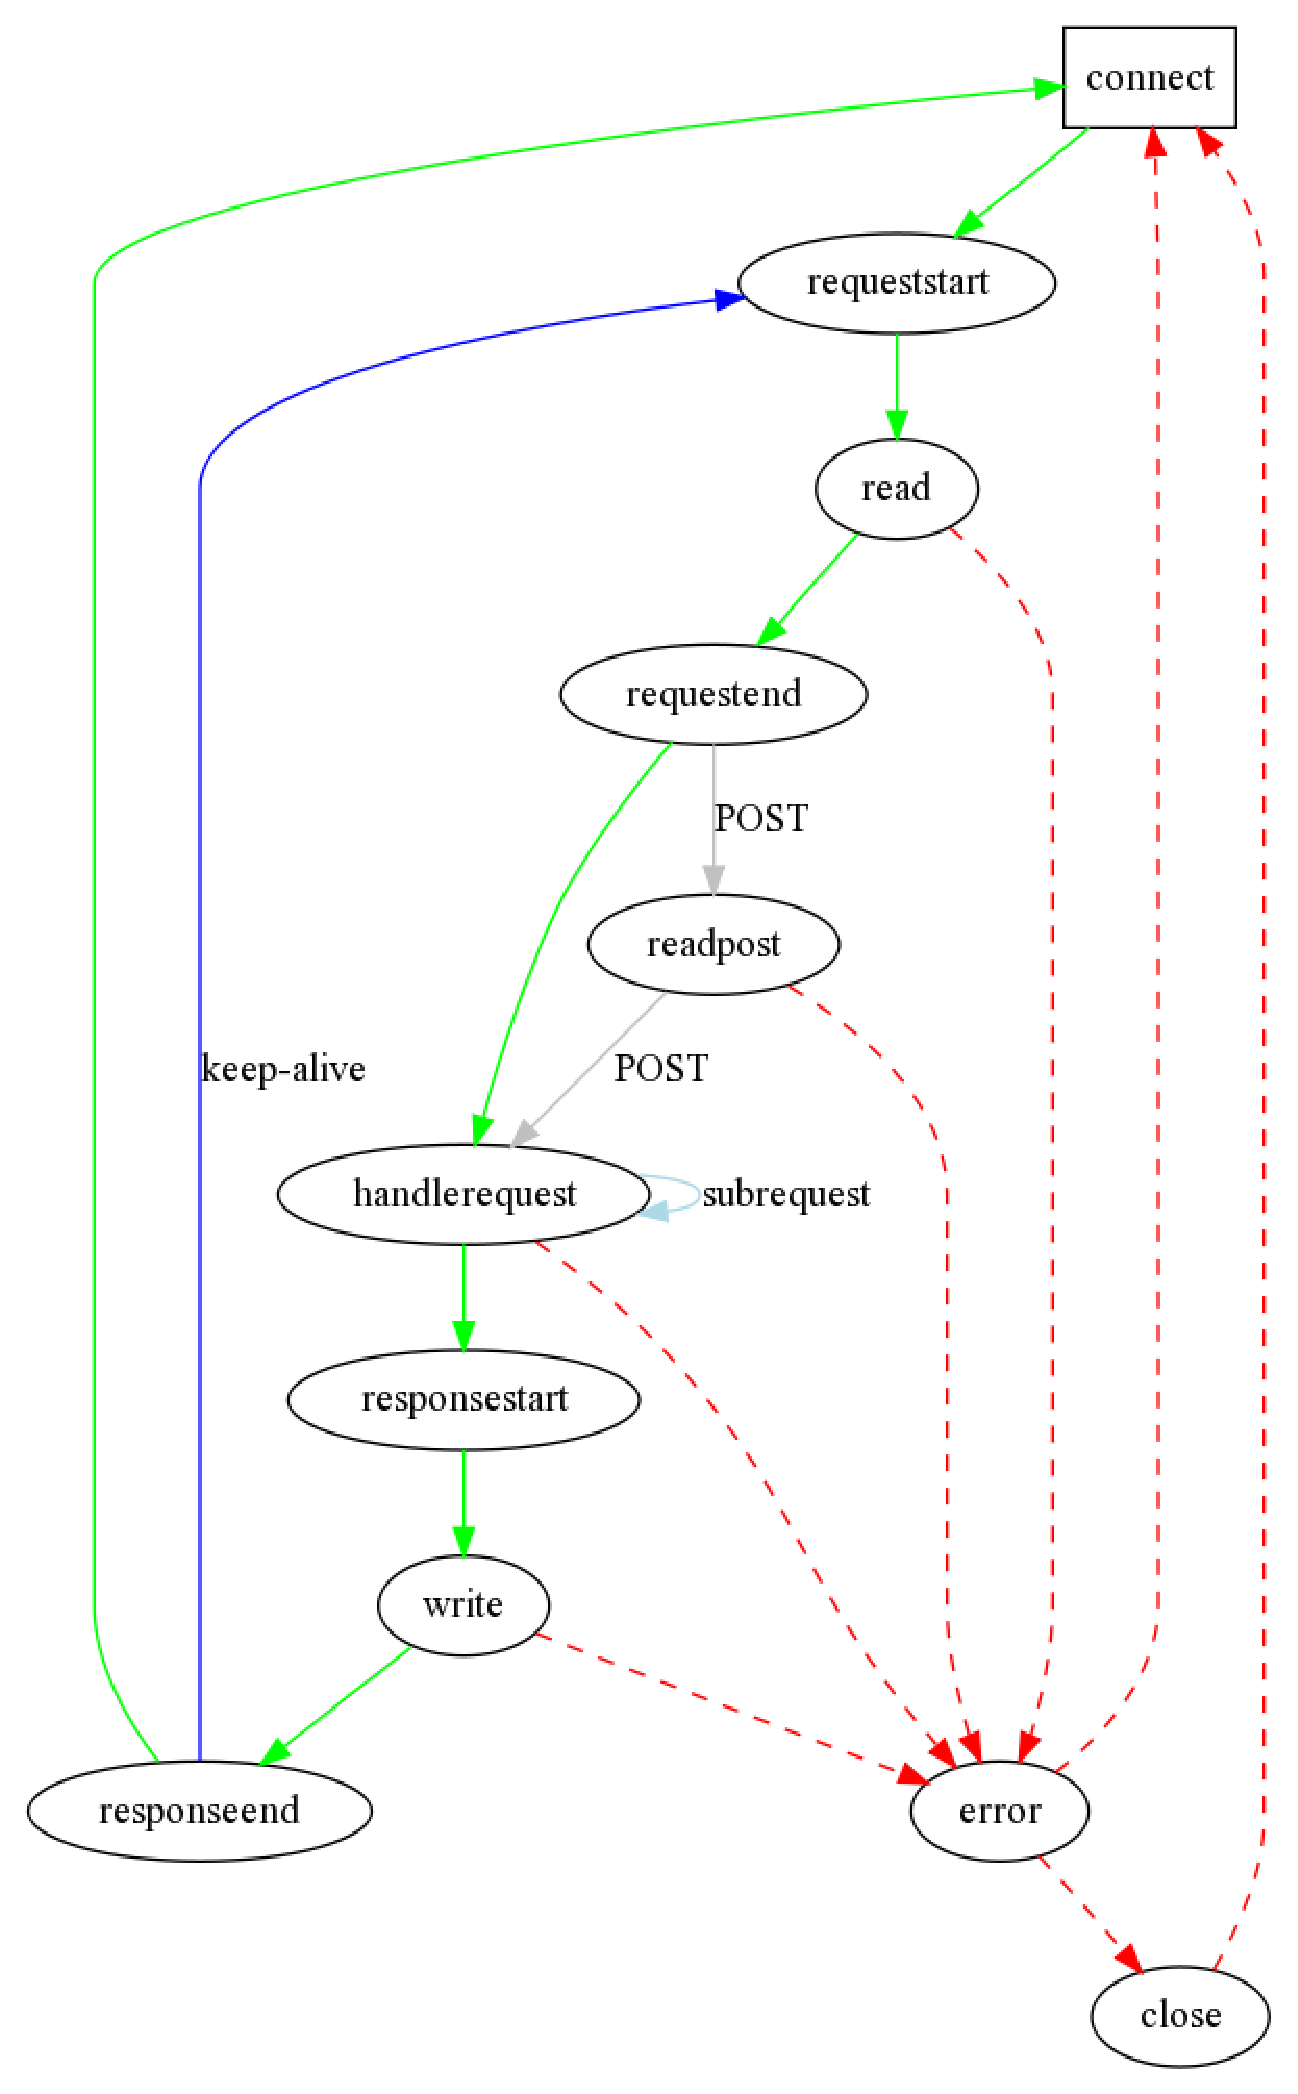
\includegraphics[height=8cm, width=6cm]{state.eps}
		\end{figure}
	\end{column}
	
	\begin{column}{0.3\textwidth}
		\begin{block}{}
			\textcolor{green}{绿色路径}为一个正常的处理路径。\\
		\end{block}
		\begin{block}{}
			\textcolor{red}{红色路径}为出错路径。\\
		\end{block}
		\begin{block}{}	
			\textcolor{blue}{蓝色路径},HTTP/1.1中保持连接。
		\end{block}
	\end{column}
	
	\end{columns}
	
\end{frame}

\section{运行结果}

\begin{frame}
	\frametitle{运行结果}
	\begin{center}
	{\Large
		七、运行结果
	}
	\end{center}
\end{frame}

\begin{frame}
	\frametitle{运行结果}
\end{frame}

\begin{frame}
	\frametitle{运行结果}
\end{frame}

\begin{frame}
	\frametitle{结束}
	\begin{center}
	{\Huge
		That's all!
	}
	\end{center}
\end{frame}

\end{document}
